\documentclass[tikz]{standalone}
\begin{document}
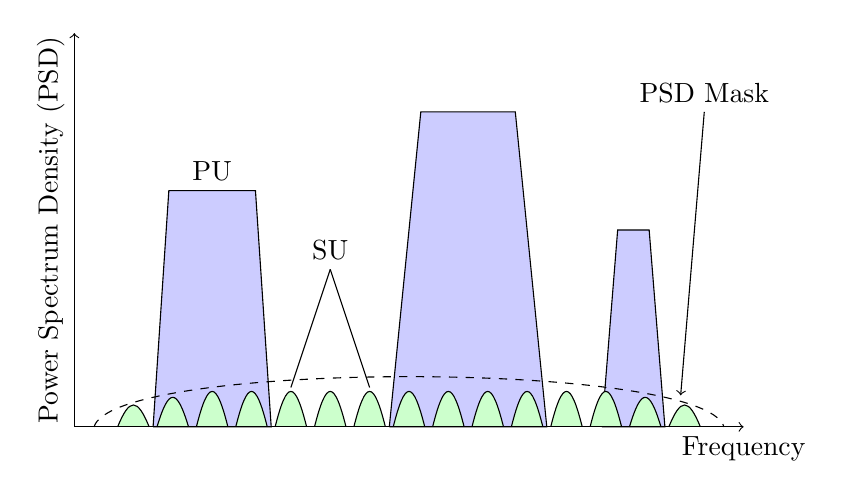
\begin{tikzpicture}
	\draw[fill=blue!20](1,0)--(1.2,3)--node[above]{PU}(2.3,3)--(2.5,0)--(1,0);
	\draw[fill=blue!20](4,0)--(4.4,4)--(5.6,4)--(6,0)--(4,0);
	\draw[fill=blue!20](6.7,0)--(6.9,2.5)--(7.3,2.5)--(7.5,0)--(6.7,0);
	\draw[dashed](0.25,0)..controls(0.5,0.85)and(8,0.85)..(8.25,0);
	\draw[fill=green!20](0.55,0)..controls(0.7,0.37)and(0.8,0.37)..(0.95,0);
	\draw[fill=green!20](1.05,0)..controls(1.2,0.5)and(1.3,0.5)..(1.45,0);
	\draw[fill=green!20](1.55,0)..controls(1.7,0.6)and(1.8,0.6)..(1.95,0);
	\draw[fill=green!20](2.05,0)..controls(2.2,0.6)and(2.3,0.6)..(2.45,0);
	\draw[fill=green!20](2.55,0)..controls(2.7,0.6)and(2.8,0.6)..(2.95,0);
	\draw[fill=green!20](3.05,0)..controls(3.2,0.6)and(3.3,0.6)..(3.45,0);
	\draw[fill=green!20](3.55,0)..controls(3.7,0.6)and(3.8,0.6)..(3.95,0);
	\draw[fill=green!20](4.05,0)..controls(4.2,0.6)and(4.3,0.6)..(4.45,0);
	\draw[fill=green!20](4.55,0)..controls(4.7,0.6)and(4.8,0.6)..(4.95,0);
	\draw[fill=green!20](5.05,0)..controls(5.2,0.6)and(5.3,0.6)..(5.45,0);
	\draw[fill=green!20](5.55,0)..controls(5.7,0.6)and(5.8,0.6)..(5.95,0);
	\draw[fill=green!20](6.05,0)..controls(6.2,0.6)and(6.3,0.6)..(6.45,0);
	\draw[fill=green!20](6.55,0)..controls(6.7,0.6)and(6.8,0.6)..(6.95,0);
	\draw[fill=green!20](7.05,0)..controls(7.2,0.5)and(7.3,0.5)..(7.45,0);
	\draw[fill=green!20](7.55,0)..controls(7.7,0.37)and(7.8,0.37)..(7.95,0);
	\draw(2.75,0.5)--(3.25,2)node[above]{SU};
	\draw(3.25,2)--(3.75,0.5);
	\draw[<-](7.7,0.4)--(8,4)node[above]{PSD Mask};
	\draw[->](0,0)--(8.5,0)node[below]{Frequency};
	\draw[->](0,0)--node[above,rotate=90]{Power Spectrum Density (PSD)}(0,5);
\end{tikzpicture}
\end{document}